\chapter{Theoretical Foundations and Motivations}\label{chap:theory}
% finish summary after writing
\textit{This chapter provides a theoretical background and motivation for the QCD multijet measurements presented in this dissertation. Quantum Chromodynamics (QCD) describes the interactions of particles with the strong force within the Standard Model (SM). The SM is a phenomenological and mathematical description of content of visible matter and three out of the four known fundamental forces. Section \ref{sec1:sm} will give a general overview of the SM. Section \ref{sec2:mc} will focus on monte-carlo event generators, particularly on the modeling of jets through parton showering and hadronisation. Finally, we will discuss current limitations of standard model calculations and simulations in Section \ref{sec3:limits} that help to motivate this measurement.}
% \vspace{-5pt}
\section{The Standard Model}\label{sec1:sm}
The Standard Model (SM) is a relativistic Quantum Field Theory (QFT) that describes three fundamental forces: the electromagnetic force, the weak nuclear force, and the strong nuclear force, and the elementary particles that make up all matter in the universe. Since its establishment by the verification of the existence of quarks in the SU(3) description in the mid 70's \cite{aitchisonhey}, it has been successful in describing and predicting the elementary particles that make up our universe, and has been extended to include the latest experimentally verified results. Figure \ref{fig:SMtikz} shows the 17 fundamental (point-like and non-composite) particles we have discovered so far comprising the SM. The fundamental interactions that govern the SM are the strong, weak, and electromagnetic forces.
\begin{figure}
    \centering
    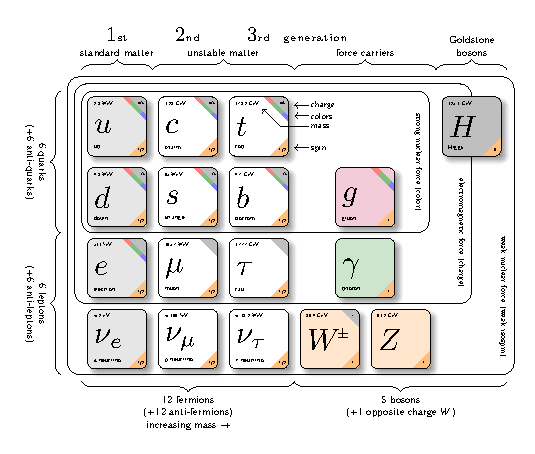
\includegraphics[width=\linewidth]{figures/SMtikz (2).pdf}
    \caption{Standard model}
    \label{fig:SMtikz}
\end{figure}
The SM 
\begin{equation}
\text{SU}(3)_C \times \text{SU}(2)_L \times \text{U}(1)_Y
\end{equation}
%Add Lagrangian
\subsection{A closer look at QCD}\label{sec1.1:ch1:QCD}
\subsection{In context}
In the context of a hadron collider, the case we are considering, there are additional non-perturbative affects that must be considered.
\section{Event Generation}\label{sec2:mc}
\subsection{}
\section{Limitations of the Standard Model and its Simulation}\label{sec3:limits}
The standard model is a "low energy" theory. Due to its perturbative nature it is only valid at a certain energy scale; in practice, after the initial collision. 
